\chapter{Interval Arithmetic}
We design an SMT solver named raSAT~\footnote{\url{http://www.jaist.ac.jp/~mizuhito/tools/rasat.html}} to solve polynomial constraint. 

Although an $O.T$ refinement loop is enough to implement an ICP based SMT solver, 
we extend it as {\bf raSAT} (SAT by refinement of approximations) loop to accelerate SAT detection 
by adding $U.T$, which works as in Fig.~\ref{fig:OTrefine}~(b). 
\begin{enumerate}
\item When an over-approximation theory $O.T$ detects $O.T$-UNSAT (resp. $O.T$-valid), 
answer UNSAT (resp. SAT). 
\item When an under-approximation theory $U.T$ detects $U.T$-SAT, answer SAT. 
\item If neither holds, a refinement is applied. 
\end{enumerate}

Our design of an SMT solver {\bf raSAT} applies two heuristic features. 
\begin{itemize}
\item Incremental widening intervals, and incremental deeping search 
(Section~\ref{sec:incsearch}). 
\item 
Heurstic measures {\em SAT-likelyhood} and {\em sensitivity}, 
for selection of a variable to decompose and a box to explore. 
(Section~\ref{sec:SATheuristics}). 
\end{itemize} 

{\bf raSAT} also prepares various interval arithmetic as $O.T$ as in Section~\ref{sec:approximation}, 
whereas currently only random tesing (\emph{k-random ticks}, 
which consists of periodical $k$-test instances with a random offset) is prepared as $U.T$. 

A typical theory for $O.T$ and $U.T$ are an interval arithmetic and testing, respectively. 
We say {\em IA-valid}, {\em IA-SAT}, and {\em IA-UNSAT}, when it is $O.T$-valid, $O.T$-SAT, and 
$O.T$-UNSAT, respectively. 
Similarly, we say {\em test-SAT} and {\em test-UNSAT}, when it is $U.T$-SAT and $U.T$-UNSAT, respectively. 
Note that either IA-valid or test-SAT implies SAT, and IA-UNSAT implies UNSAT, 
whereas IA-SAT and test-UNSAT can conclude neither. 


%We instantiate testing to $U.T$ in Section~\ref{sec:raSATloop}. 
%%%%%%%%%%%%%%%%
\suppress{
\begin{definition}\label{def:testing}
%For $\exists x_1 \in (a_1,b_1) \cdots x_n \in (a_n,b_n). \bigwedge \limits_{i=1}^m f_i(x_1,\cdots,x_n) > 0$, 
Let $M = \bigwedge \limits_{i=1}^m x_i \in (a_i,b_i)$ and 
${\mathcal P} = \bigwedge \limits_{i=1}^m f_i(x_1,\cdots,x_n) > 0$. 
%
Let a choice function $\theta : (\Real \times \Real)^n \rightarrow \Real^n$ 
such that $\theta(M) \in (a_1,b_1) \times \cdots \times (a_n,b_n)$. 
Testing is a finite set $\Theta$ of choice functions. Then, we say 
\begin{itemize}
\item ${\mathcal P}$ is \emph{Test-SAT} under $M$ if $\theta(M)$ holds ${\mathcal P}$ 
for some $\theta \in \Theta$, and 
\item ${\mathcal P}$ is \emph{Test-UNSAT} under $M$ if $\theta(M)$ never holds ${\mathcal P}$ 
for each $\theta \in \Theta$. 
\end{itemize} 
%We denote $I \models_{test(\theta)} P$ if $\bigwedge \limits_{i=1}^m f_i(\theta(I)) > 0$ holds.
\end{definition}
}
%%%%%%%%%%%%%%%%


{\bf raSAT} prepares various Affine intervals, adding to classical interval (CI)~\cite{moore}, 
which keep lower and upper bounds. The weakness of CI is loss of dependency 
among values. For instance, $x - x$ is evaluated to $(-2,2)$ for $x \in (2,4)$. 

Affine Interval~\cite{af,comba93} introduces \emph{noise symbols} $\epsilon$, 
which are interpreted as values in $(-1,1)$. 
For instance, $x = 3 + \epsilon$ describes $x \in (2,4)$, and 
$x - x = (3 + \epsilon) - (3 + \epsilon)$ is evaluated to $0$. 
The drawback is that the multiplication without dependency might be less precise than CI.
Affine intervals also cannot represent infinite intervals, e.g., $(0,\infty)$, 
since it becomes $\infty + \infty~\epsilon$. 
Forms of affine intervals vary by choices how to approximate multiplications. They are,
\begin{enumerate}[(i)]
\item $\epsilon \epsilon'$ is replaced with a fresh noise symbol 
($AF$)~\cite{StolfiThesis,comba93}, 
\item $\epsilon \epsilon'$ is reduced to the fixed error noise symbol 
$\epsilon_{\pm}$ ($AF_1$ and $AF_2$) \cite{af},
\item $\epsilon \epsilon'$ is replaced with $(-1,1) \epsilon$ 
(or $(-1,1) \epsilon'$) ($EAI$)~\cite{ngocsefm},
\item $\epsilon \epsilon$ is reduced to fixed noise symbols 
$\epsilon_+$ or $\epsilon_{-}$ ($AF_2$) \cite{af}, 
\item Chebyshev approximation of $x^2$ introduces a noise symbol $|\epsilon|$ 
as an absolute value of $\epsilon$ with 
$\epsilon \epsilon = |\epsilon| |\epsilon| = |\epsilon| + (-\frac{1}{4}, 0)$ and
$\epsilon |\epsilon| = \epsilon + (-\frac{1}{4}, \frac{1}{4})$ \cite{tapas12}. 
%(Fig.~\ref{fig:chevabs}). 
%\item keeping products of noise symbols up to degree $2$ ($\epsilon_i \epsilon_j$),
\end{enumerate} 

%%%%%%%%%%%%%%%%%
\suppress{
\begin{remark}
For Affine intervals, \emph{sensitivity}~\cite{ngocsefm} of a variable
is a possible range of the absolute value of the coefficient of its corresponding $\epsilon$. 

%In Example~\ref{examp:sensitivity}, $CAI$ estimates the coefficient of $|\epsilon_1|$ as $\textbf{3}$, 
%which has the largest sensitivity and indicates $x$ the most influencial. 

Note that Affine interval works only for bounded intervals. 
For instance, $\infty + \infty \epsilon$ represents $(-\infty,\infty)$, which says nothing. 
Narrowing intervals as an incremental search (Section~\ref{sec:incsearch}) partilly depends on this fact. 
That is, if $\pm \infty$ is contained in an interval, first give finite upper/lower bounds and search 
within these bounds using an Affine interval. If UNSAT is concluded, then enlarge to the whole intervals 
using CI. 
\end{remark}
}
%%%%%%%%%%%%%%%%%


\begin{example} \label{examp:sensitivity}
Let $f = x^3 - 2xy$ with $x = (0,2)$ ($x = 1 + \epsilon_1$) and $y=(1,3)$ ($y = 2+\epsilon_2$), 
we have,
\begin{itemize}
\item $AF_2$ estimates the range of $f$ as 
$-3 - \epsilon_1 - 2\epsilon_2 + 3\epsilon_+ + 3\epsilon_{\pm}$, thus $(-9,6)$,
\item $CAI$ estimates the range of $f$ as 
$(-4,-\frac{11}{4}) + (-\frac{1}{4}, 0)\epsilon_1 - 2\epsilon_2 + \textbf{3}|\epsilon_1| + (-2,2)\epsilon_{\pm}$, 
thus $(-8,4.5)$.
\end{itemize}
\end{example}



%%%%%%%%%%%%%%%%%%%%%%%%%%
\suppress{
\begin{figure}[ht]
\begin{minipage}[b]{1.0\linewidth}
\centering
\begin{tabular}{ll}
\includegraphics[height=1.6in,width=1.7in]{chev1.pdf} &
\includegraphics[height=1.6in,width=1.7in]{chev2.pdf}
\end{tabular}
\caption{Chebyshev approximation of $x^2$ and $x~|x|$}
\label{fig:chevabs}
\end{minipage}
\end{figure}

$CAI$ \cite{tapas12} consists of (ii) and (v), which keeps better precision than iv)
for multiplicatins of the same variables, e.g., Taylor expansion. 
%To improve precision in estimating upper and lower bounds of polynomials, we apply 
%\textbf{Affine Arithmetic} such as $AF_1$, $AF_2$ \cite{af}, $CAI$ ~\cite{tapas12} 
%instead of Classical Interval \cite{moore}. 
%Note that upper and lower bounds estimated by IA are over-approximation bounds of polynomials.

}
%%%%%%%%%%%%%%%%%%%%%%%%%%
\suppress{
\begin{definition}
%For $\exists x_1 \in (a_1,b_1) \cdots x_n \in (a_n,b_n). \bigwedge \limits_{i=1}^m f_i(x_1,\cdots,x_n) > 0$, 
Let $M = \bigwedge \limits_{i=1}^m x_i \in (a_i,b_i)$ and 
${\mathcal P} = \bigwedge \limits_{i=1}^m f_i(x_1,\cdots,x_n) > 0$. 
%
Let $\delta_i^l$ and $\delta_i^u$ be lower and upper bounds of $f_i(x_1,\cdots,x_n)$ 
estimated by IA for $x_i \in (a_i,b_i)$. Then, we say 
%
%\vspace*{0.5em}
\begin{itemize}
\item ${\mathcal P}$ is \emph{IA-VALID} under $M$, if IA evaluates 
$~\forall i \in [1,m].~\delta_i^l > 0$,
%\vspace*{0.33em}
\item ${\mathcal P}$ is \emph{IA-UNSAT} under $M$, 
$~\exists i \in [1,m].~\delta_i^u \leq 0$, and 
\item ${\mathcal P}$ is \emph{IA-SAT} under $M$, if 
$(\exists j \in [1,m].~\delta_j^l \leq 0)\; \wedge \; 
	(\bigwedge \limits_{i=1}^m \delta_i^u > 0)$.
\end{itemize} 
\end{definition}

IA-VALID and IA-UNSAT safely reason satisfiability (SAT) and unsatisfiability (UNSAT), 
respectively. However, IA-SAT cannot conclude SAT. 
}


\suppress{
I. Selecting API for testing:
  (1) Difficulty first by SAT-likelihood.   
  (2) Easy first by SAT-likelihood
  (10) Random.,
II. Selecting Variable:
  (8) With sensitivity
  (9) Without sensitivity - Random: 
III. Selecting box:
  (3) SAT-directed using IA-Testing.
  (4) UNSAT-directed using IA-Testing.
  (5) SAT-directed using SAT-likelihood
  (6) UNSAT-directed using SAT-likelihood
  (7) Random
}


\begin{figure}[ht]
%\begin{minipage}[b]{1.0\linewidth}
\centering
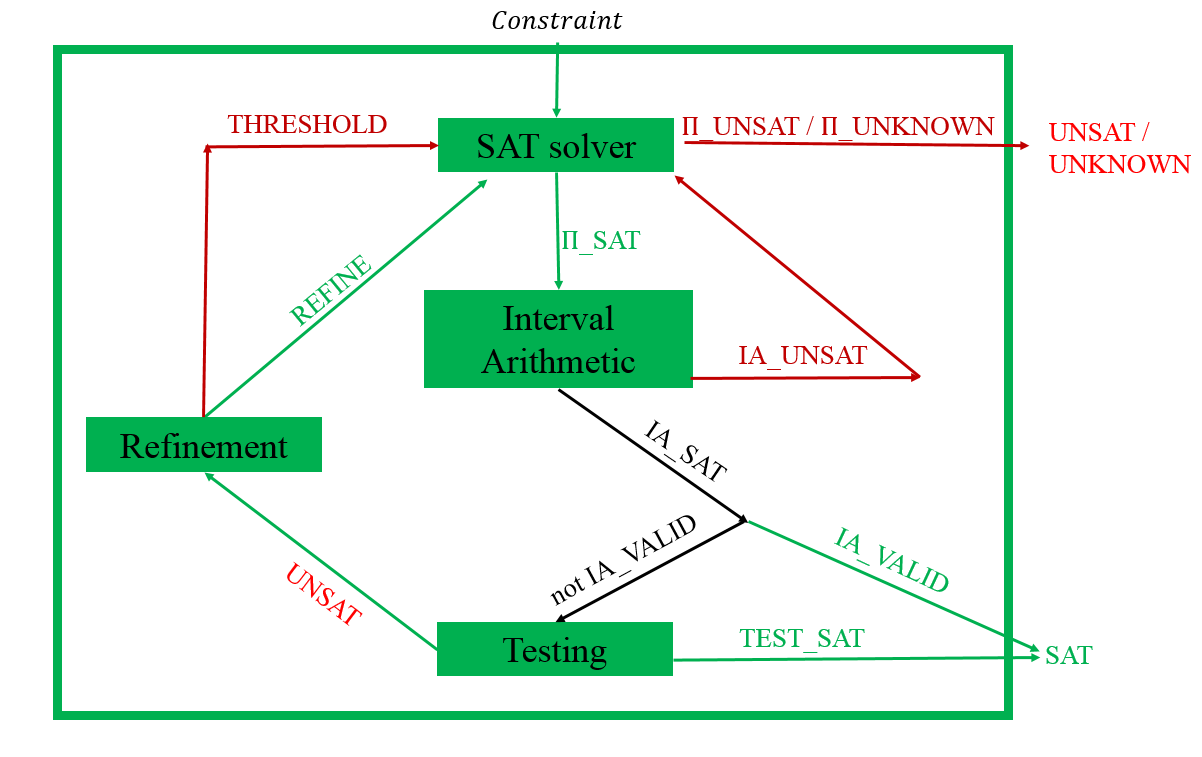
\includegraphics[width=\textwidth]{smt-design.png} 
\caption{\textbf{raSAT} design} 
\label{fig:smt-design} 
%\end{minipage}
\end{figure} 